\chapter{Testbeam experiment at FNAL}

Testbeam experiment provides a controlled environment in which detectors are exposed to particle beams that mimics real experimental conditions. The experiment is required for evaluating the performance of prototype detector modules prior to their installation in large-scale experiments such as CMS. The following sections present the beam facility, experimental configuration and key physics considerations relevant to the study.

\section{The Fermilab Test Beam Facility}

The Fermilab Test Beam Facility (FTBF), located in Batavia, Illinois, is a high-energy accelerator facility dedicated to testing and developing particle detectors for experiments such as CMS. It delivers a primary beam of $120\,\text{GeV}$ protons at variable intensities (1--300\,kHz), extracted in controlled spills approximately every 60 seconds.

The beam is formed by a sequence of accelerators: $750\,\text{keV}$ H$^-$ ions are first accelerated initially in the Linear Accelerator (Linac) to $400\,\text{MeV}$, then injected into the Booster where electrons are stripped and protons are accelerated to $8\,\text{GeV}$. These protons are transferred to the Main Injector and boosted to $120\,\text{GeV}$. The extracted beam is then routed through the Fermilab Switchyard, which splits and directs it to experimental areas, including the Meson Test Beam Facility (MTest) and the Meson Center Beam Facility (MCenter). Secondary and tertiary beamlines can also be created by placing absorbers and targets into the primary beamline. These consist of muons, pions, or electrons, with energies as low as $1\,\text{GeV}$ for the secondary beamline and down to $200\,\text{MeV}$ for the tertiary beamline. A schematic of the beamline is shown in Figure~\ref{fig:fermi_complex}.

\begin{figure}[H]
    \centering
    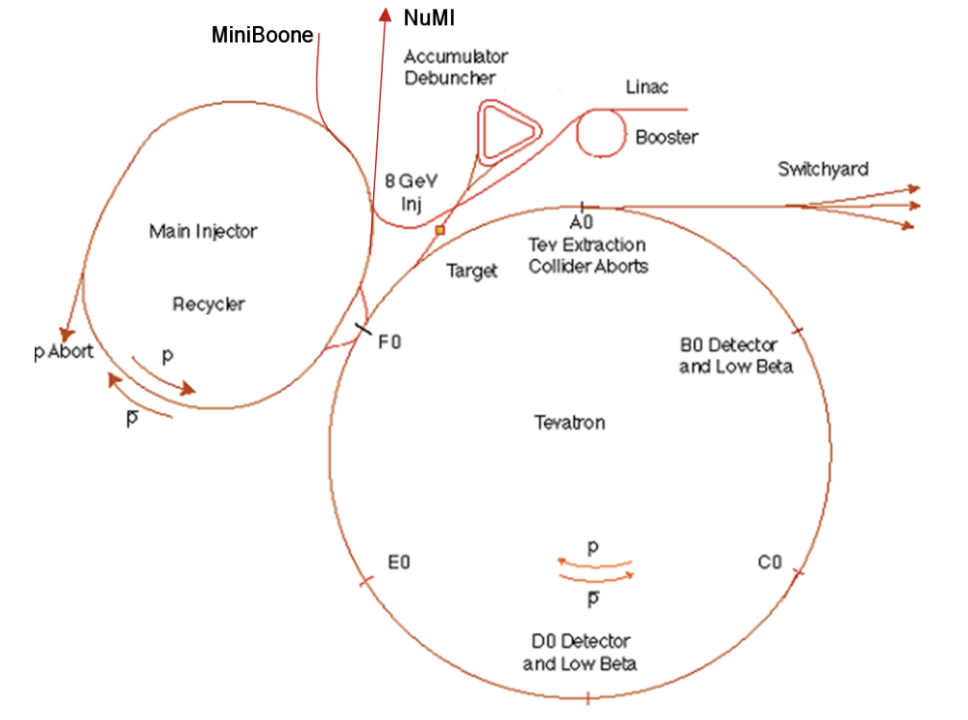
\includegraphics[width=0.8\textwidth]{images/Fermilab_accelerator.png}
    \caption{Schematic layout of the Fermilab accelerator complex \cite{Stephen_Holmes_2011}.}
    \label{fig:fermi_complex}
\end{figure}

A silicon pixel tracking telescope is permanently installed in MTest to provide high-resolution tracking of beam particles Fermilab also hosts the Irradiation Test Area (ITA), which is used for controlled radiation studies of detector components under HL-LHC-like conditions.

\section{Telescope Infrastructure and Alignment}

The tracking telescope at FNAL is designed to sustain high-precision measurements of the Device Under Test (DUT). The telescope includes six silicon strip planes positioned upstream, where two pairs of planes are arranged orthogonally to each other to improve resolution by measuring the X and Y positions of hits. Downstream of the DUT, four pixel planes are placed together with the same six strip planes, as shown in Figure~\ref{fig:telescope}. The pixel sensors employ $100 \times 150 \times 320~\mu\text{m}^3$ cells and cover an active area of approximately $1.6 \times 1.6~\text{cm}^2$, achieving a resolution of about $8~\mu\text{m}$ due to the tilted sensor geometry. The strip detectors provide even better resolution, approximately $5~\mu\text{m}$, with a pitch of $60~\mu\text{m}$ and an active area on the order of $3.8 \times 3.8~\text{cm}^2$ \cite{KWAN2016162}.

\begin{figure}[H]
    \centering
    \includegraphics[width=1\textwidth]{images/telescope.png}
    \caption{FNAL telescope structure.}
    \label{fig:telescope}
\end{figure}

The primary beam within the MTest area traverses three scintillators placed upstream and one scintillator downstream of the pixel telescope. The coincidence of these scintillators creates a signal that starts the data acquisition for the entire detector arrangement. A unique identifier is assigned to each trigger so that data from the pixel planes, strip detectors, and DUT possible be arranged into a single unit referred to as an "event". Track reconstruction up to frequencies of about 40 kHz is supported by the system while maintaining trigger information integrity. In addition to trigger numbers, timestamps are saved to allow offline synchronization of the telescope and DUT data streams.

Data acquisition is controlled by the Compact And Programmable daTa Acquisition Node (CAPTAN), a system developed at Fermilab \cite{Adam_2019}. The telescope consists of three independent stations, each containing a CAPTAN module. The central module, which is also connected to the DUT, mantained as the master module and synchronizes data taking in the whole system. All modules are linked to the control room computer, where data is recorded and monitored over the operational time.

Telescope alignment is performed offline using the Monicelli program. It begins with the reconstruction of tracks using a chi-squared fit of the hit positions, with cluster positions given by charge-weighted averages if there are multiple pixels. Monicelli then iteratively adapts the telescope geometry to minimize the residuals in the transverse directions for each pixel plane. The optimal geometry, characterized by the minimum residuals, is selected. This arrangement, together with the fixed position of the DUT, allows the beam position at the DUT to be determined correctly.

\section{Planar sensor structure and physics properties}

The Testbeam experiment's planar silicon sensors are produced by Hamamatsu Photonics K.K. (HPK) and are tested as a component of the DUT within the telescope setup. The sensors are intended to be bump-bonded with CMS Readout Chips (CROCs). Two pixel sensor dimensions, to be standardized for the HL-LHC, are presented in Figure~\ref{fig:pixel_sensors}.

\begin{figure}[H]
    \centering
    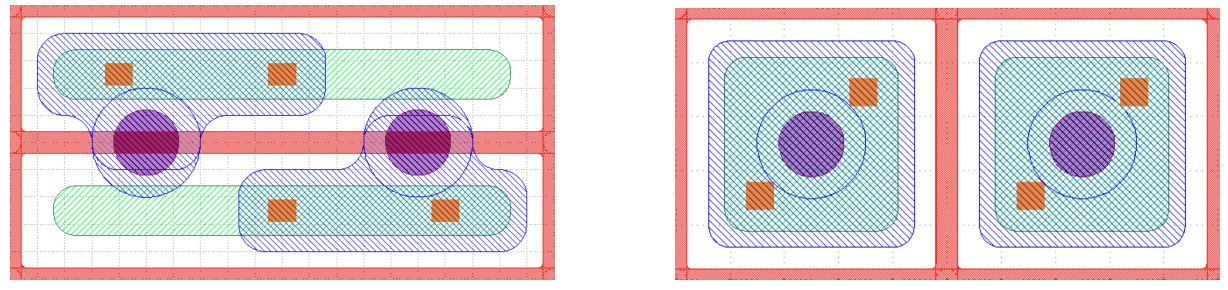
\includegraphics[width=1\textwidth]{images/pixels.png}
    \caption{Layout of two pixel cells of the HPK sensor submission: $25 \times 100~\mu\text{m}^2$ (left) and $50 \times 50~\mu\text{m}^2$ (right). The $n^+$ implants are shown in green, metal layers in blue, $p$-stop regions in red, contacts in orange, and bump bond pads in purple \cite{CERN-LHCC-2017-009}.}
    \label{fig:pixel_sensors}
\end{figure}

Silicon semiconductors are fundamental for particle detectors due to the small band gap which allow ionization radiation such as a MIP to remove electrons from valence zone generating electron-hole pairs and typically deposits around 80 $e$--$h$ pairs per micrometer of sensor thickness.

\begin{figure}[H]
    \centering
    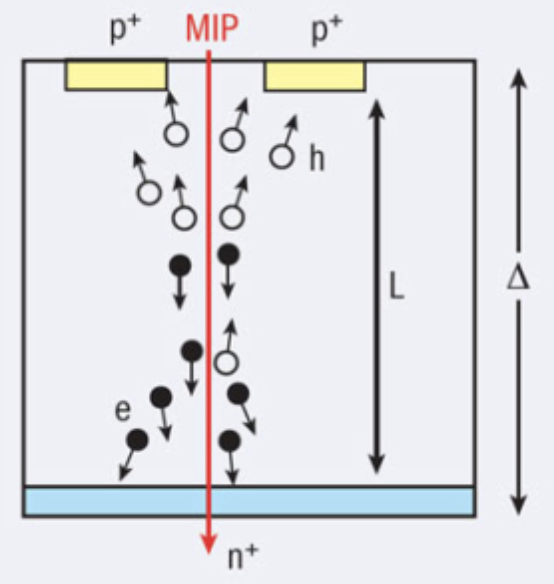
\includegraphics[width=0.4\textwidth]{images/planar_sensor.png}
    \caption{Schematic cross-section of a planar sensor design, illustrating how the active thickness ($\Delta$) and the charge collection distance ($L$) are independently defined.}
    \label{fig:planar_sensor}
\end{figure}

When a reverse bias voltage ($V_{\text{bias}}$) is applied across the $p^+$--$n^+$ junction, it depletes the free charge carriers from the bulk of the sensor, generating an electric field $\vec{E}$ which extends into the active thickness $\Delta$. When the depletion region extends throughout the entire sensor, the sensor becomes fully depleted. The drift of the holes and electrons under the influence of the electric field induces a current, which is picked up by the readout chips. The total charge $Q$ from a traversing particle can be estimated by:
\begin{equation}
    Q = q \cdot \frac{dE}{dx} \cdot \Delta,
\end{equation}
where $q$ is the elementary charge, $dE/dx$ s the particle's energy loss per unit path length. Its variation with the momentum of the particle is given by the Bethe-Bloch equation, which is plotted in Figure~\ref{fig:Bloch}. The curve indicates how the stopping power of charged particles changes with their energy and drops to a minimum value known as minimum ionization. Most particles formed by high-energy collisions pass through silicon sensors in this regime, releasing a very uniform amount of energy, and thus the response of the detector is known and reproducible.

For optimum performance, the sensor is biased slightly above full depletion in order to reduce the leakage current and prevent breakdown. Leakage current rises with voltage as:
\begin{equation}
    I_{\text{leak}} \propto \sqrt{V_{\text{bias}}},
\end{equation}
up to full depletion, then rising steeply, at which breakdown begins.

Figure~\ref{fig:planar_sensor} is a schematic of a planar sensor geometry with an MIP generating $e$--$h$ pairs, which are subsequently separated by the electric field and collected at the opposite electrodes, inducing a detectable signal.

\begin{figure}[H]
    \centering
    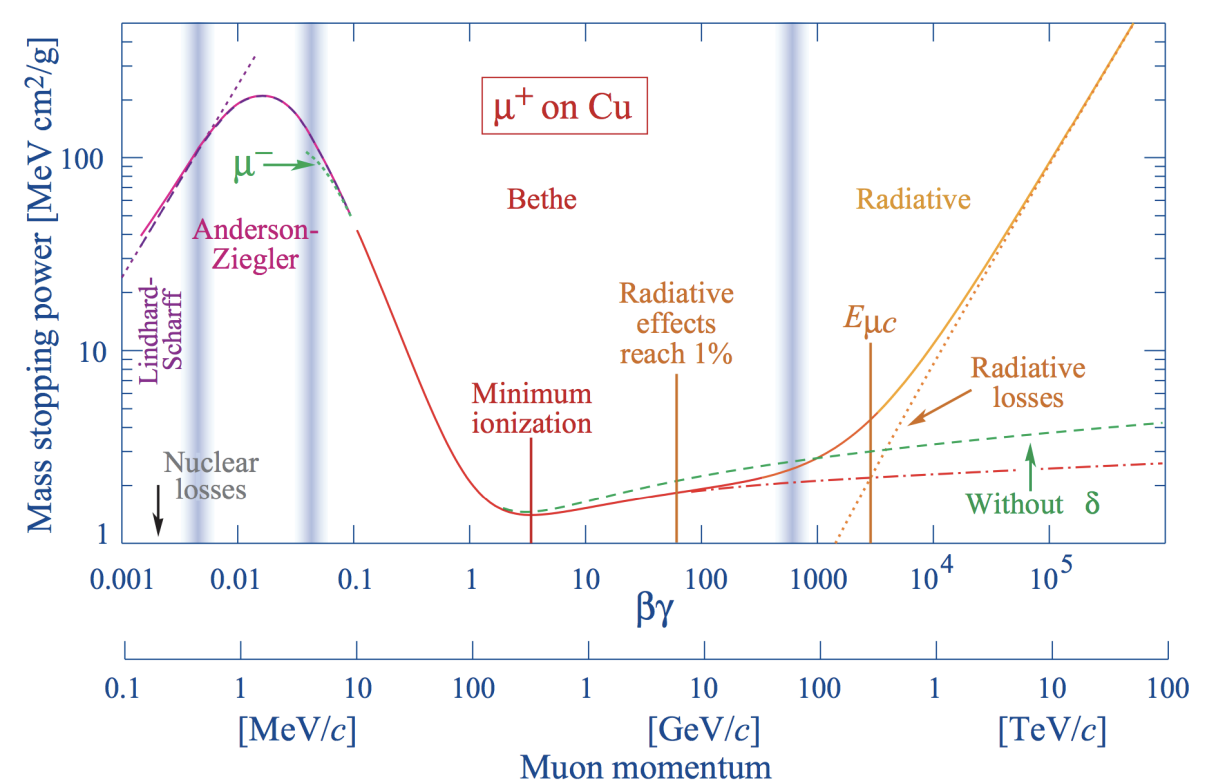
\includegraphics[width=0.9\textwidth]{images/Bloch.png}
    \caption{Mass stopping power ($-\frac{dE}{dx}$) for muons in copper as a function of $\beta\gamma = \frac{p}{mc}$ (bottom axis) and momentum (top axes), showing the Bethe-Bloch behavior. The curve is a plateau at minimum ionization, rising at high energy from radiative losses. This behavior produces the minimum ionizing particles (MIPs) energy loss in silicon-based tracking detectors \cite{Bichsel200827PO}.}
    \label{fig:Bloch}
\end{figure}

\section{Sensor Response Effects}
\subsection{Radiation Damage}

The radiational damage of silicon sensors is critical for the efficiency of the detector for the HL-LHC. The damage may take the form of crystal lattice defects (bulk damage) or surface damage due to interactions with insulating layers. These effects result in higher leakage currents, deformation of the electric field distribution, and charge trapping—all resulting in inefficient charge collection. Furthermore, radiation damage will raise the electronic noise, which can be partly eliminated by selecting a suitable readout threshold \cite{Eber_2014}.

\subsection{Charge Charing}

When a charged particle (such as a MIP) traverses a silicon sensor, it produces electron-hole pairs along its trajectory. The charge carriers are subsequently separated and drift under the influence of an electric field toward the collecting electrodes. If the particle passes near the boundary between two neighboring pixels, the resulting charge cloud may spread due to diffusion—particularly in the transverse direction—or be displaced by Lorentz drift in the presence of a magnetic field. As a result, both electrodes may collect a portion of the charge, leading to what is known as charge sharing.

\subsection{Crosstalk}

Crosstalk is the result of unintentianal signal coupling between adjacent pixels which leads to a degradation of the spatial resolution and misreconstruction of hits.

In Figure~\ref{fig:xtalk_layout}, a top perspective of a pixel layout demonstrates coupling between metal lines of neighboring pixels which is a common source of capacitive crosstalk.

\begin{figure}[H]
    \centering
    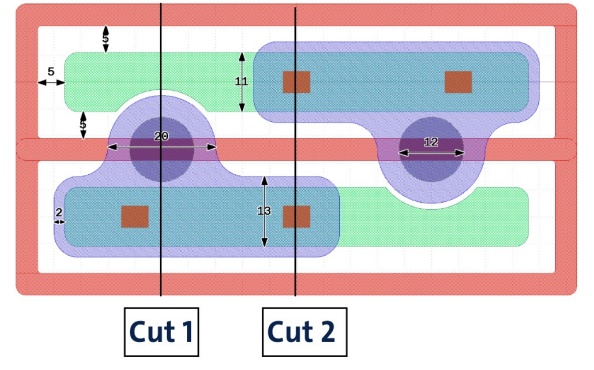
\includegraphics[width=0.5\textwidth]{images/RH0017.png}
    \caption{Top view of the pixel cell layout showing n$^+$ implants (green), metal lines (blue), p-stop structures (red), and passivation layers. The proximity of metal traces across neighboring pixels can give rise to capacitive crosstalk.}
    \label{fig:xtalk_layout}
\end{figure}

Figure~\ref{fig:xtalk_cut} illustrates vertical cuts (Cut 1 and Cut 2) of the pixel cell structure. The lack of any type of shielding or isolation structures in steps as such may result in a signal going through one pixel coupling to the neighboring pixel.

\begin{figure}[H]
    \centering
    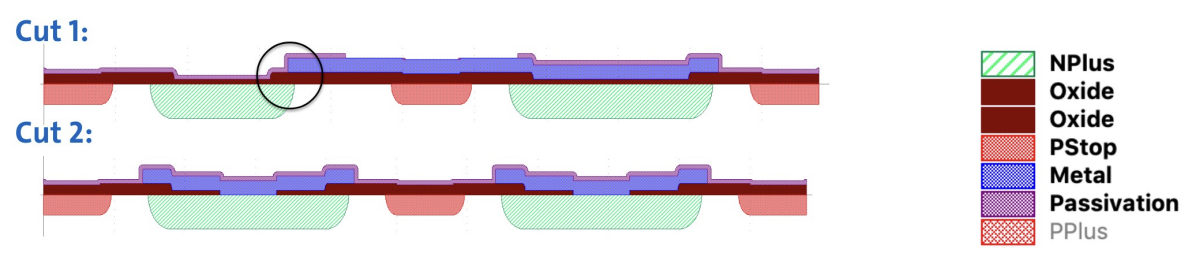
\includegraphics[width=0.8\textwidth]{images/RH0017cut.png}
    \caption{Cross-sectional views (Cut 1 and Cut 2) of the pixel sensor illustrating different vertical layouts. In Cut 1 the metal layer can increase capacitive coupling between adjacent pixels, leading to crosstalk.}
    \label{fig:xtalk_cut}
\end{figure}

Good shielding and layout practices are needed to minimize crosstalk.

\subsection{Delta rays}

Delta rays are secondary electrons of high energy knocked out of atoms during irradiation by a fast charged particle. They shift far from the parent track and generate further ionization, creating electron-hole pairs on trajectories other than the central one. The charge deposition can thus extend to the adjacent pixels, causing more charge sharing and in general forming larger or asymmetrical clusters. The photons can additionally distort charge patterns and complicate track reconstruction, particularly in high-precision pixel detectors.
